\documentclass[french,a4paper]{article}
\setcounter{tocdepth}{4}
\setcounter{secnumdepth}{4}
\usepackage{float}
\usepackage{graphicx}
\newcommand{\tabitem}{\textbullet~~}
\usepackage{multirow}
\graphicspath{{img/}}
\title{PPII}
\usepackage[bottom=2.5cm,top=2.5cm,left=2.5cm,right=2.5cm]{geometry}
\author{Noé Steiner - Alexis Marcel - Lucas Laurent - Mathias Aurand-Augier}
\date{Octobre 2022}
\begin{document}

\maketitle
\newpage
\tableofcontents
\newpage
\section{Contexte du projet}
Ce rapport rend compte du Projet Pluridisciplinaire d’Informatique Intégrative dans le cadre de la première année du cycle ingénieur à TELECOM Nancy.
L’objectif de ce projet est de concevoir, en groupe,  une application dédiée à l’optimisation des ressources dans les vergers et potagers partagés du territoire.

\newpage
\section{Etat de l'art}
\subsection{Introduction}
Les enjeux climatiques n’ont jamais été aussi élevés. Notre planète arrive à la fin de ses énergies fossiles. Les ressources deviennent rares, les changements climatiques provoquent des pénuries, des sécheresses et des catastrophes naturelles. Le mode de vie que nous connaissons aujourd’hui doit changer et devenir plus écoresponsable. L’objectif est de changer les habitudes de consommation de produits venants du monde entier en se restreignant à une zone géographique bien plus petite. La politique actuelle serait de privilégier les produits de notre pays mais essayons d’aller plus loin…

En effet, un mode de vie plus judicieux écologiquement serait de revenir à des productions locales en passant directement par les producteurs. Certaines personnes ont une surface de production ( jardin, verger) mais n’ont pas le temps ou les moyens de s’en occuper. Tandis que d’autres personnes, n’ont pas de terrain mais sont prêtes à donner de leur temps pour pouvoir consommer localement.

Notre solution~: utiliser les technologies modernes du web pour proposer une application permettant à n’importe qui de créer/rejoindre un jardin mais surtout de pouvoir gérer facilement un jardin sur lequel plusieurs personnes vont agir.

\subsection{Définition d’un circuit court et d’un jardin partagé}
\subsubsection{Qu’est ce qu’un circuit court ?}

\textbf{Le circuit court est une pratique de commercialisation des produits agricoles consistant à limiter au maximum le nombre d’intermédiaires (en général 0 ou 1) entre le producteur et le consommateur.} Il établit donc une proximité à la fois géographique, mais également relationnelle entre le producteur et le consommateur.

Si aucun intermédiaire n’existe, on parle alors de vente directe. Elle permet notamment à l’agriculteur de mener son activité en toute indépendance, de fixer les prix qu’il désire sans laisser de commission à un quelconque tiers.

Dans l’optique de vendre leurs produits, les agriculteurs d’une même région peuvent créer un partenariat de type AMAP (Association pour le Maintien de l'Agriculture Paysanne) basé sur un système de distribution de paniers  composés des produits de la ferme (éventuellement fromage, viande, légume, fruit, oeuf) et ainsi offrir une diversité importante de produit de saison. Ils peuvent également utiliser d'autres réseaux tels que la Ruche qui Dit Oui, ou encore Bienvenue à la ferme. Mais il existe également d’autres alternatives de vente tels que les drives fermiers qui consistent pour les agriculteurs à proposer leurs produits fermiers en ligne, avec le retrait de la commande dans un point de retrait. Il peut également vendre ses produits par l’intermédiaire de coopératives ou de magasins bio (directement en contact avec le producteur) ou simplement stand dans les marchés du dimanche.

Durant le printemps 2020 et le confinement, les producteurs ont été de plus en plus nombreux à vendre en circuits courts. Malgré cela, la vente directe ne représente aujourd’hui que 5 à 10\% de la consommation alimentaire totale en France.
\subsubsection{Qu’est ce qu’un jardin partagé ?}
\textbf{Un jardin partagé est un jardin conçu, construit et cultivé collectivement par les habitants d’un quartier.} La création de jardin partagé repose aujourd’hui sur l’initiative des habitants. C’est un projet de quartier associant confiance, convivialité et entraide. Le but étant que chaque membre du jardin participe quotidiennement à sa gestion. Ce procédé rentre ainsi directement dans le principe de circuit court. 

L’émergence des jardins partagés remonte au 19ème siècle lors de la révolution industrielle. En effet, les populations essentiellement rurales se sont dirigées vers les villes pour trouver du travail. Cependant, les conditions de vie y étaient précaires et les jardins partagés appelés  “jardins ouvriers” étaient un moyen de survie. De ce fait, lors de la première guerre mondiale, les jardins partagés ont connu un essor conséquent. Dans les années 1970, suite au développement économique, les jardins partagés connaissent un déclin majeur, la population n'en éprouvant plus le besoin.

Au fil le temps, le développement de la mondialisation a favorisé l’importation en grande quantité au détriment de la production à l’échelle locale favorisant la qualité des produits. Ce mode de fonctionnement en circuit long a pris de plus en plus de place dans notre quotidien. 

Cependant, les conditions climatiques et le manque de qualité sont en train d'inciter les citoyens recommencer à privilégier les circuits courts tels que les jardins partagés.

\subsubsection{L'émergence des jardins partagés ?}

En 2021, le gouvernement a lancé un appel aux projets de jardins partagés dans le cadre du programme France Relance. Par cet appel, le gouvernement propose des aides financières aux organismes voulant mettre en place des jardins partagés. De nombreux projets de jardins partagés ont déjà été mis en place grâce à cet appel.
\begin{figure}[H]
    \centering
    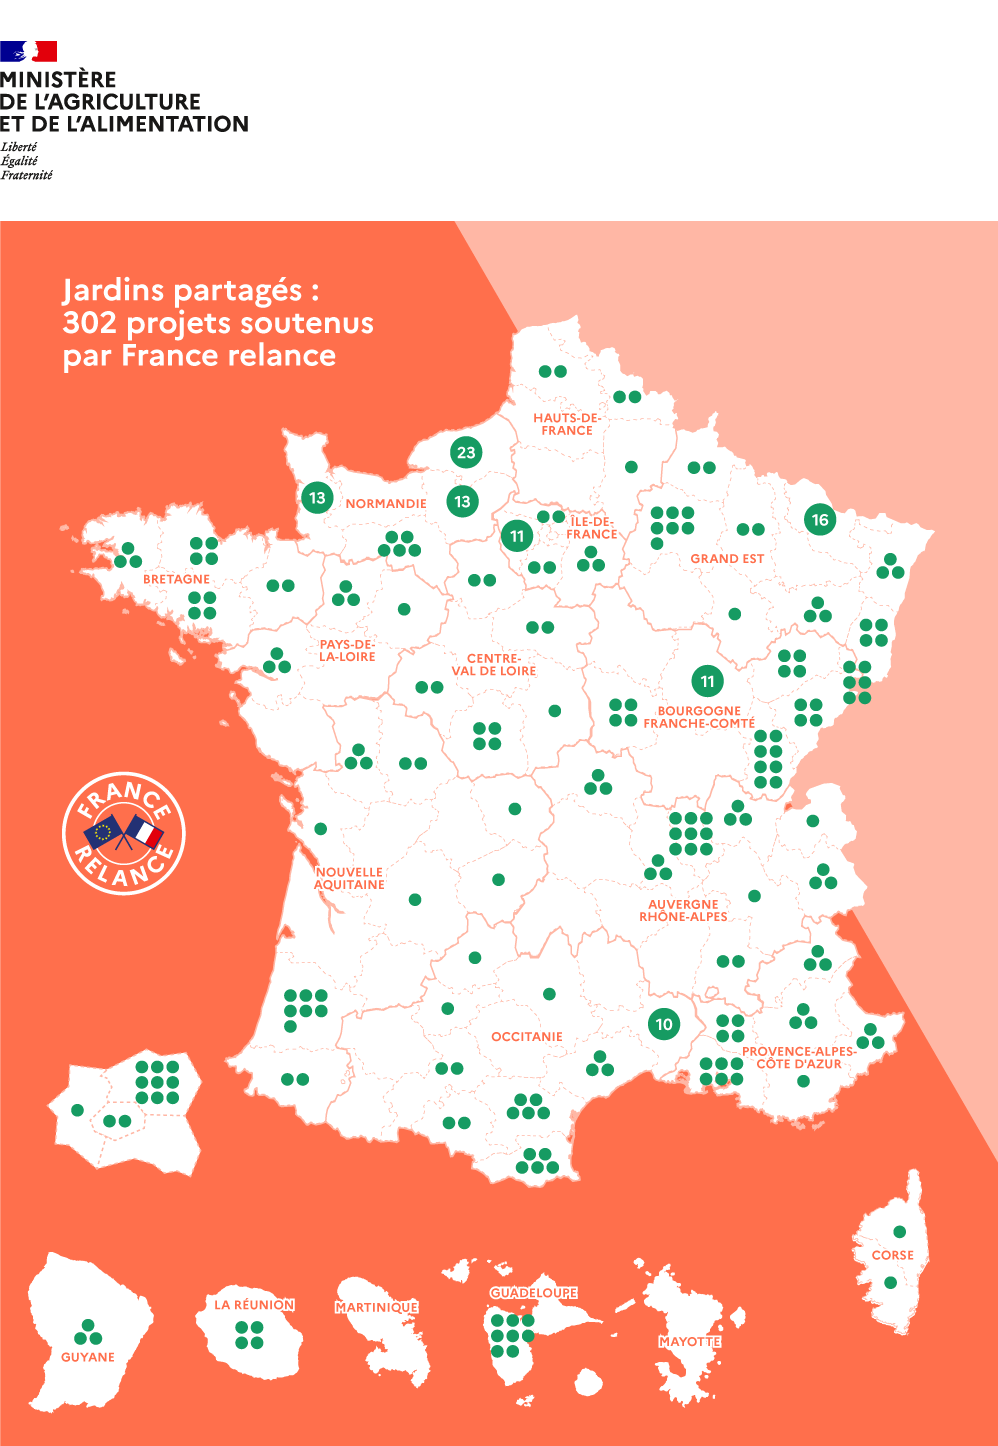
\includegraphics[width=0.5\textwidth]{img/francerelance_carte.png}
    \caption{Jardins partagés en France}
\end{figure}
Le concept de jardin partagé est aujourd’hui en plein essor et la population, soutenue par le gouvernement, s’investit de plus en plus dans une démarche de consommation en circuit court. 

C’est pourquoi notre projet s’inscrit précisément dans la tendance actuelle en favorisant les circuits courts et en permettant à des personnes de faire le pas dans le monde des jardins partagés. Le but de ce projet est notamment de  permettre la gestion d’un tel jardin partagé.

\subsection{Les jardins partagés et les technologies}
De nombreuses applications conernant les jardins existent. 
Cependant, elles permettent en général soient~: de gérer les plantes de son jardin, soit de créer/rejoindre des jardins partagés.

Nous avons ainsi répertorié ces applications existente en classant leurs fonctionnalités principales dans un tableau~:

\begin{center}
    \begin{tabular}{ |l| p{3cm} | p{3cm} | p{3cm} | p{3cm} | }
        \hline
                         & \raggedright création de jardin public (visible sur la carte) & \raggedright Création de jardin privée (disponible sur lien d’invitation) & \raggedright Gestion globale du jardin & Gestion précise du jardin en organisation de tâche par parcelle \\
        \hline
        Groww            &                                                              &                                                                            & x                                      &                                                                 \\
        \hline
        AdopteMaTomate   & x                                                            &                                                                            &                                        &                                                                 \\
        \hline
        Pandasuite       & x                                                            &                                                                            &                                        &                                                                 \\
        \hline
        Plantezcheznous  & x                                                            &                                                                            &                                        &                                                                 \\
        \hline
        Click and garden & x                                                            &                                                                            &                                        &                                                                 \\

        \hline
    \end{tabular}
\end{center}

Groww est une application de gestion de jardin qui permet d’avoir une liste de tâches à faire en fonction de ses plantes. Cependant, ce logiciel est limité pour la gestion d’un jardin entier séparé en plusieurs parties et surtout il ne permet pas de gérer plusieurs contributeurs au jardin.

Les autres applications centrées sur le principe de jardin partagé permettent seulement de créer un jardin qui sera affiché sur une carte à l’adresse du jardin. N’importe qui peut alors faire une demande pour rejoindre le jardin en cliquant directement sur la carte. Cependant ces applications n’incluent pas la gestion du jardin, ce qui peut être très complexe à partir du moment où le jardin est partagé avec plusieurs personnes.

En effet, un jardin inclus plusieurs tâches à faire différentes en fonction de la période de l'année. De plus, il est souvent séparé en plusieurs compartiments correspondant à un type de culture séparé par des passages pour se déplacer. Un jardin géré par plusieurs personnes s'avèrent donc être un travail délicat au même titre qu'un projet de groupe sans gestion de projet. 

C’est pourquoi notre application permet non seulement de créer et de rejoindre des jardins mais également de gérer de façon détaillée le jardin. De plus, créer un jardin n’engendre pas forcément une localisation public sur la carte mais à la possibilité d'être privé et les utilisateurs peuvent le rejoindre grâce à un lien d’invitation envoyé par le créateur du jardin.


\newpage
\section{Gestion de projet}
\subsection{Équipe de projet}
Ce projet est un projet local réalisé en groupe de 4 personnes~:
\begin{itemize}
    \item Alexis MARCEL
    \item Lucas LAURENT
    \item Noé STEINER
    \item Mathias AURAND-AUGIER
\end{itemize}
Le comité de pilotage est constitué de~:
\begin{itemize}
    \item Anne-Claire HEURTEL
    \item Olivier FESTOR
    \item Gérald OSTER
\end{itemize}
Ces personnes constituent les parties prenantes de notre projet ainsi que les acteurs influents sur le livrables.
\begin{figure}[H]
    \centering
    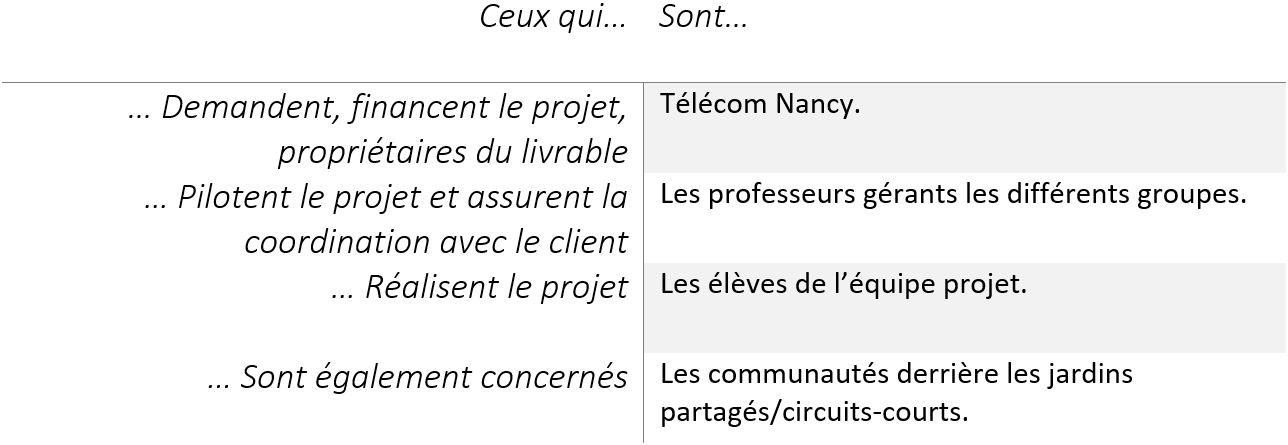
\includegraphics[width=0.75\textwidth]{img/parties_prenantes.png}
    \caption{Parties prenantes}
\end{figure} 
\subsection{Organisation au sein de l’équipe projet}
Nous avons réalisé plusieurs réunions, en présentiel dans les locaux de Télécom Nancy mais également sur en visio-conférence sur Discord. Ces réunions nous ont permis de mettre en commun nos avancés régulièrement, de partager nos connaissances sur des problématiques et de nous organiser de manière optimale.
Les comptes rendus des réunions réalisés sont présents dans l’Annexe 1.

De plus, dès le début de notre projet nous avons mis en place un projet Trello. Trello est une application permettant d’organiser facilement un projet en reposant sur une organisation en planches listant des cartes, chacune représentant des tâches. Ces tâches peuvent ensuite être déplacées permettant de découper notre projet en plusieurs jalons dynamiquement.
\begin{figure}[H]
    \centering
    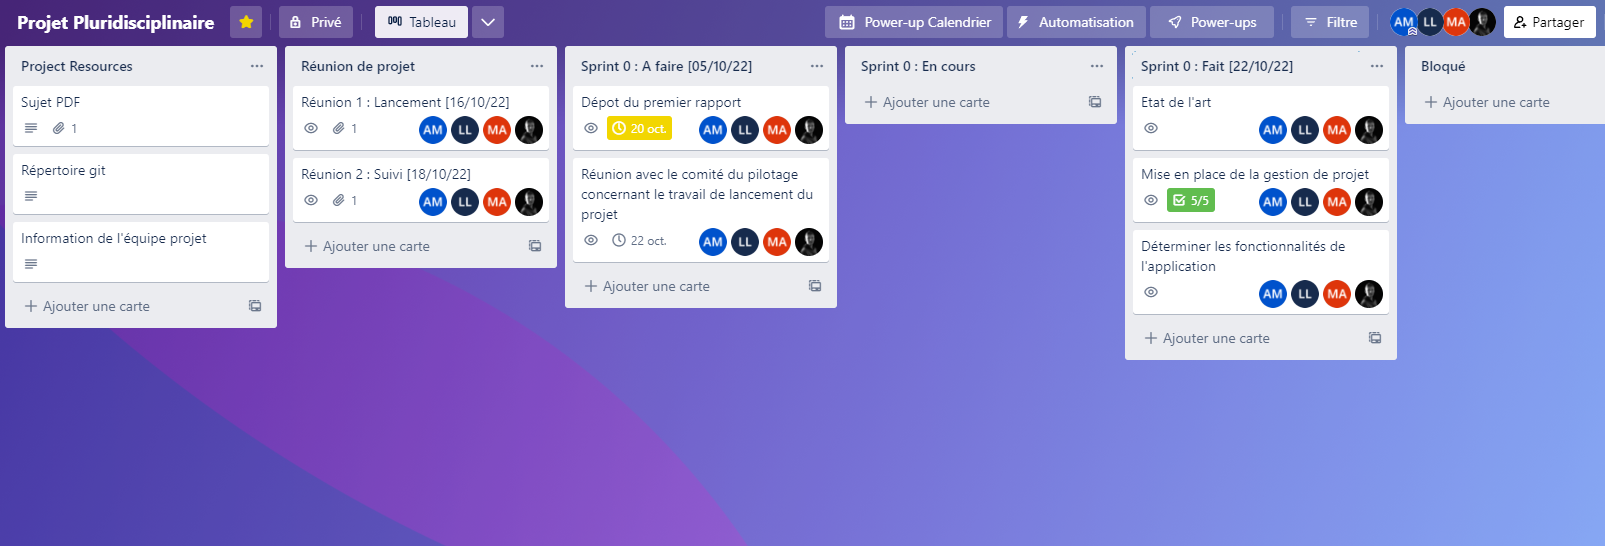
\includegraphics[width=0.75\textwidth]{img/trello.png}
    \caption{Organisation Trello}
\end{figure} 

Ensuite, nous avons utilisé GitLab pour gérer les différentes versions du développement de notre application, ainsi que les différentes branches nous permettant de travailler simultanément sans conflit.

Enfin, la rédaction des differents comptes rendu de réunion et des rapports ont été rédigé en \LaTeX.

\subsection{Triangle qualité-cout-délai}
Afin d’établir des objectifs cohérents, et réalisables dans les délais, nous avons réalisé le triangle qualité-coût-délai. On remarque ainsi, les délais étant courts, que nous avons tout intérêt à ne pas se fixer des objectifs trop ambitieux sous peine de devoir renoncer à certaines fonctionnalités et de ne pas rendre le livrable annoncé initialement.

\begin{figure}[H]
    \centering
    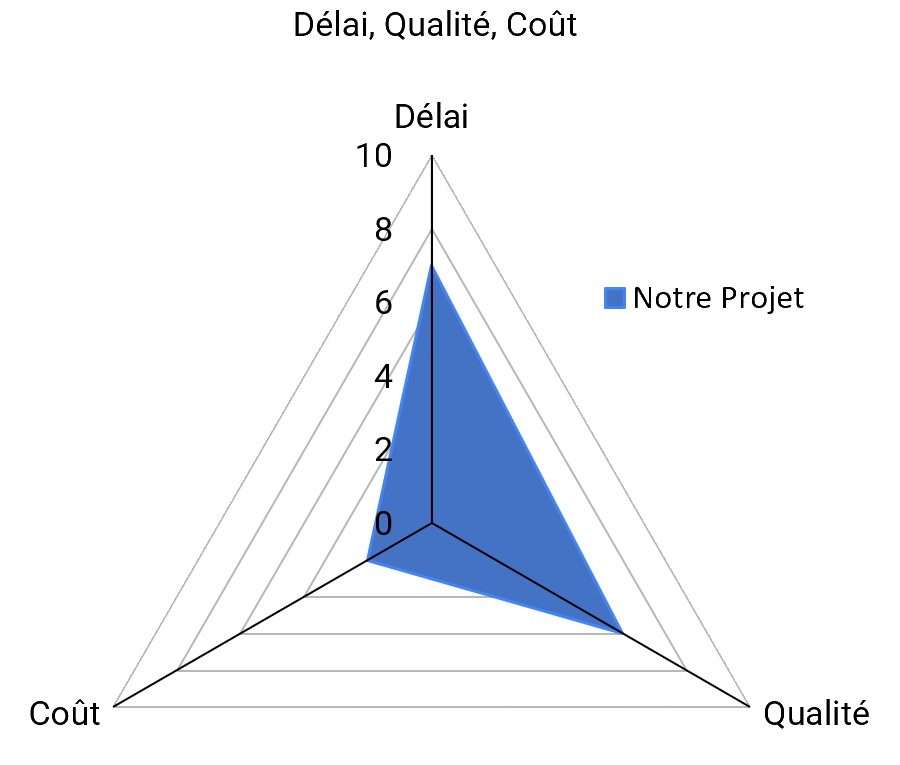
\includegraphics[width=0.5\textwidth]{img/triangle_QCD.png}
    \caption{Triangle DQC}
\end{figure} 

\subsection{Matrice SWOT}
Afin d’avoir une vision plus globale de nos ressources et des facteurs interne et externe agissant sur le projet, nous avons ensuite réalisé la matrice SWOT (Strengths, Weaknesses, Opportunities, Threats) de notre projet.

\begin{figure}[H]
    \centering
    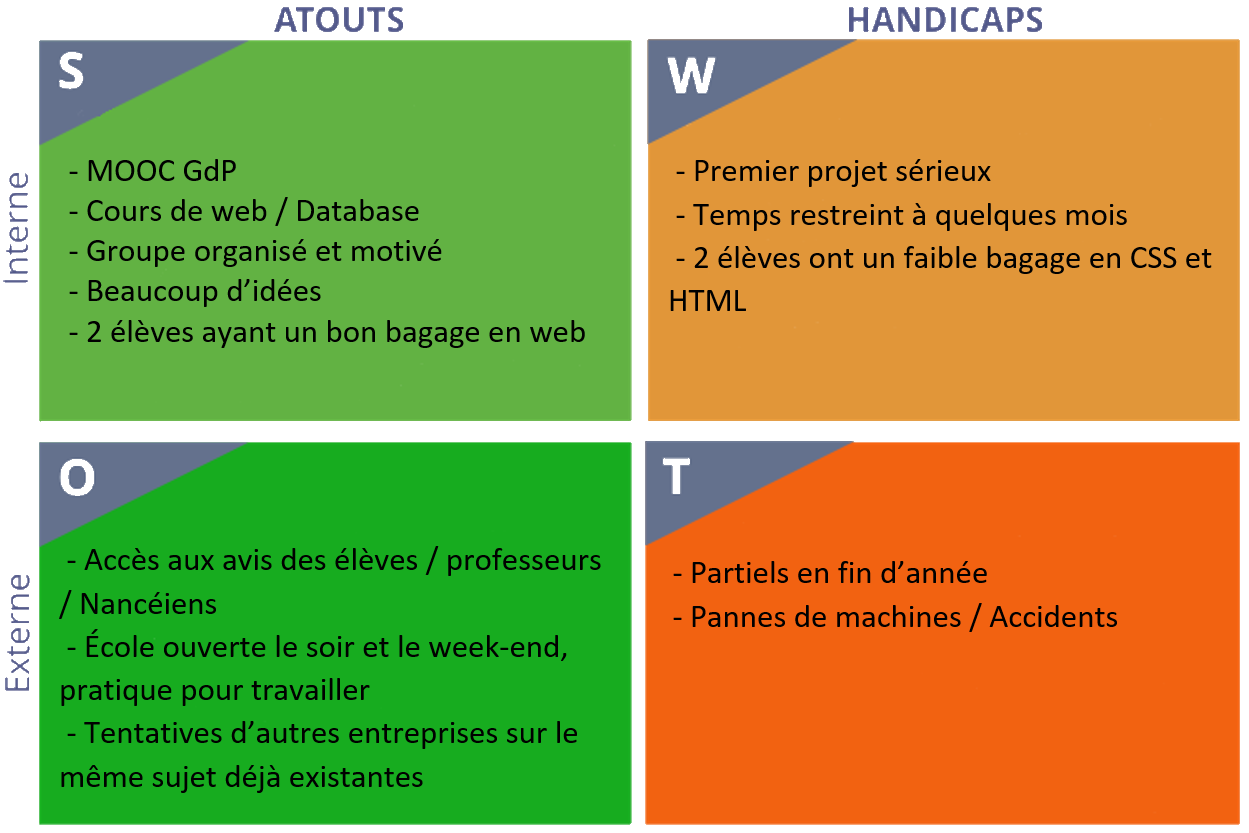
\includegraphics[width=0.75\textwidth]{img/SWOT.png}
    \caption{Matrice SWOT}
\end{figure} 

On peut ainsi remarquer que notre projet présente de nombreux points fort notamment grâce aux connaissances acquises lors des cours de Télécom Nancy mais également de part l’expérience forte de deux des membres de l’équipe projet qui ont déjà réalisé des applications similaires.  Cependant, plusieurs facteurs internes constituent nos faiblesses notamment les courts délais qui nous oblige à être concis et efficaces dans notre travail, ou encore le faible bagage informatique de deux des membres de l’équipe. Néanmoins, ces lacunes constituent pour eux l’opportunité d’apprendre, et de progresser avec l’aide des membres expérimentés de l’équipe.

De plus, nous devons anticiper les charges de travail dans le cadre de notre formation à Télécom Nancy qui s'avèrent être plus élevée en décembre lors des partiels de fin d'année. Nous allons donc devoir prendre cela en compte dans notre gestion des tâches. 

\subsection{Profil de projet}
Afin d’avoir une vision plus globale sur notre projet, nous avons également réalisé le profil du projet (le budget étant égal à 0, nous avons choisi de ne pas le représenter dans notre profil). On remarque que, du fait des nombreuses fonctionnalités que nous avons l’intention d’implémenter dans notre application, que notre projet est de taille moyenne mais de complexité élevée.

Cependant, les enjeux du projet ne sont pas très importants (en dehors de la note finale qui compte dans notre moyenne) car l'échec du projet n'engendra pas la chute d'une organisation et le budget est négligeable.

De plus, au vu de l’état de l’art établi, l’innovation du projet est importante puisque nous avons choisi de combiner différentes fonctionnalités existantes de plusieurs applications et d’en rajouter de nouvelles.

\begin{figure}[H]
    \centering
    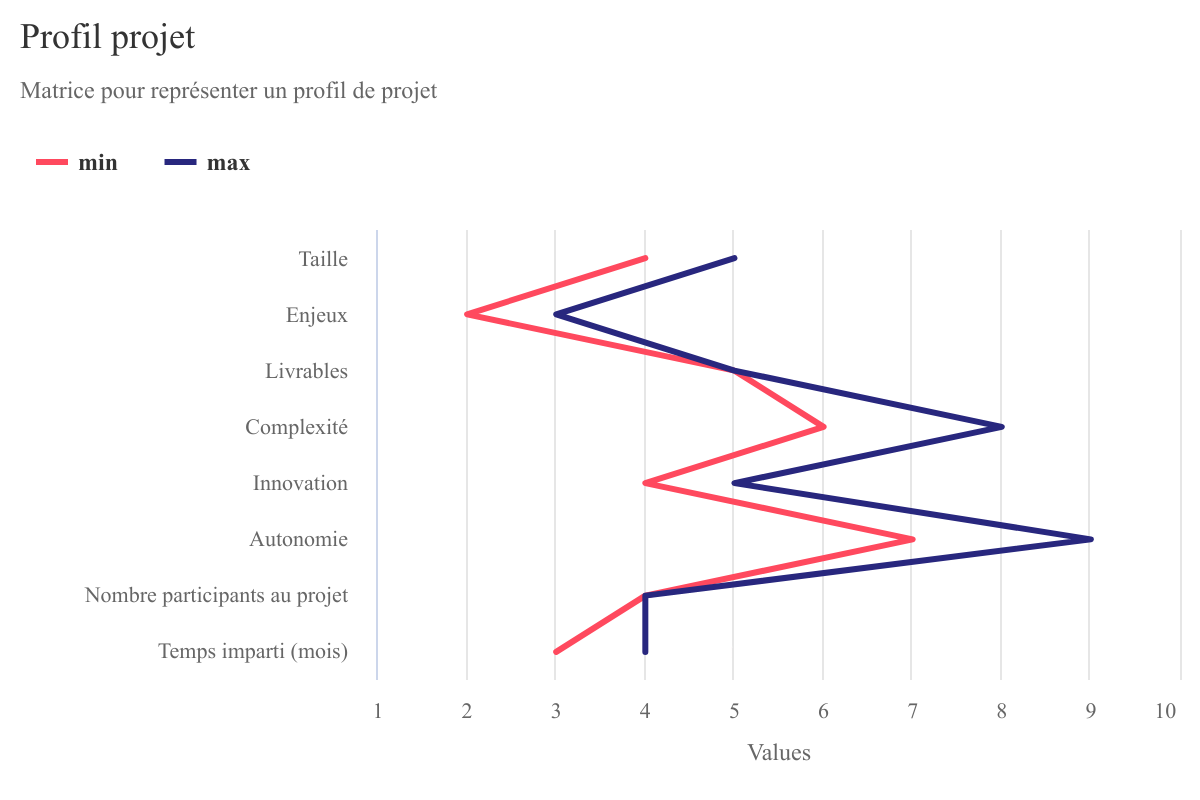
\includegraphics[width=0.75\textwidth]{img/profil_projet.png}
    \caption{Profil du projet}
\end{figure} 

\subsection{WBS~: comment concrétiser l’application}
Ceci étant fait, nous avons maintenant choisi de détailler les lots de travail à effectuer pour fabriquer notre application. Nous avons ainsi réalisé le WBS (Work Breakdown Structure) de notre application~: il apparait ainsi les grandes étapes de notre projet que sont~: definition du cadre de l’application, développement des fonctionnalités de l’application et écriture du rapport.
\begin{figure}[H]
    \centering
    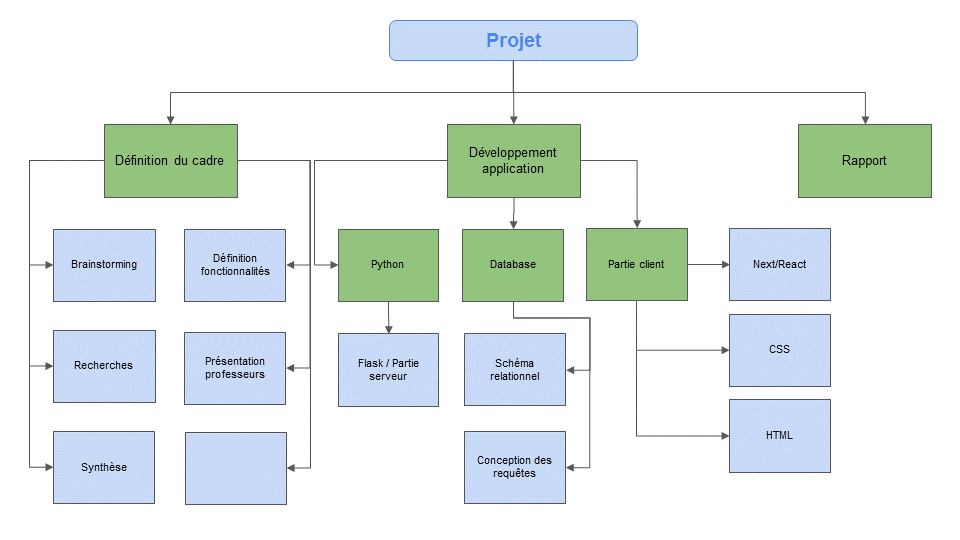
\includegraphics[width=0.75\textwidth]{img/WBS.png}
    \caption{WBS}
\end{figure} 

\subsection{Diagramme de Gantt~: planification}
Maintenant que nous avons un détail des lots de travail qui constitue notre application, il faut maintenant les mettre en relation pour créer un planning efficace où chaque tâche est effectuée dans l’ordre.
\begin{figure}[H]
    \centering
    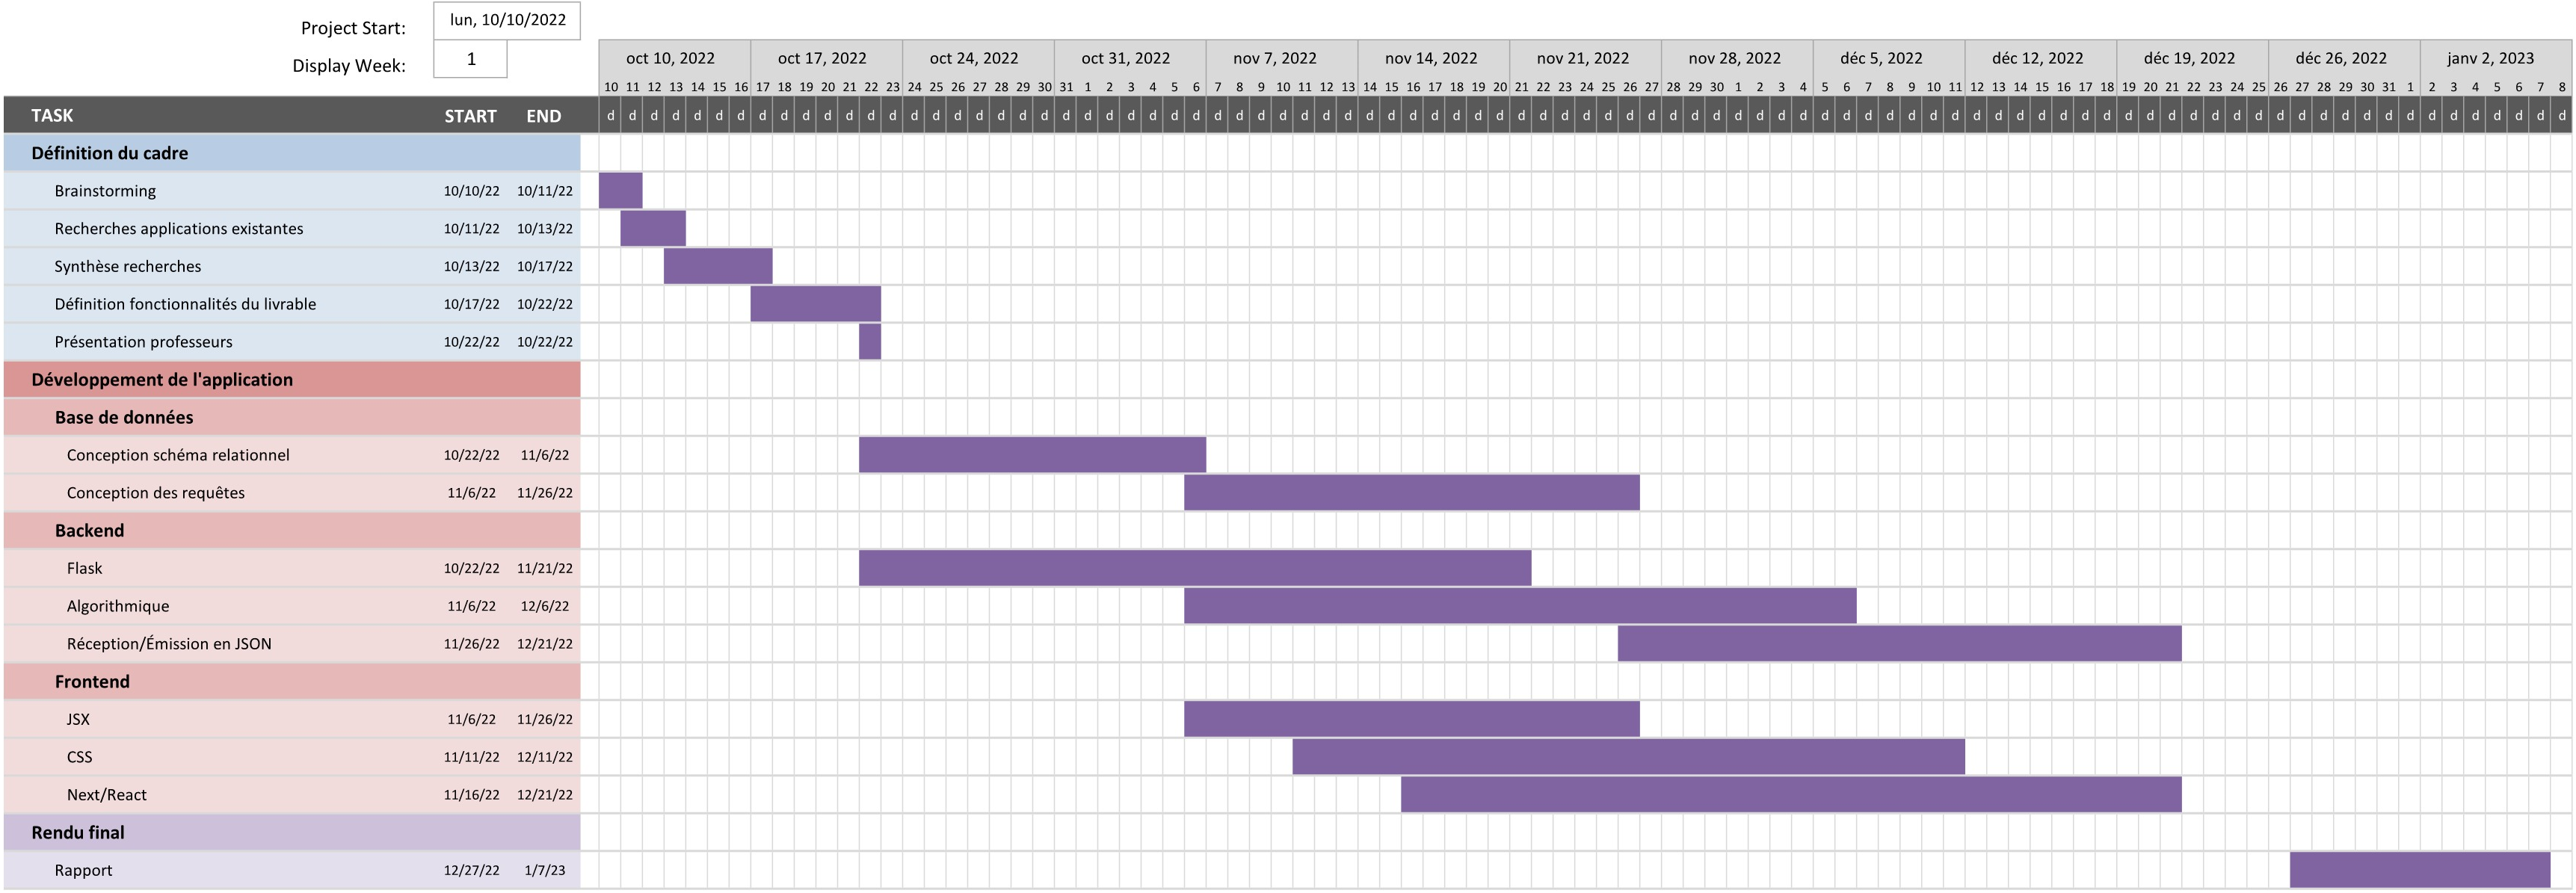
\includegraphics[width=0.9\textwidth]{img/gantt.png}
    \caption{Diagramme de GANTT}
\end{figure} 
Ce diagramme est une première version générale des tâches à effectuer, il sera modifié et détaillé davantage une fois la conception et les maquettes du projet réalisé.

\subsection{Matrice RACI}
Maintenant que toutes les étapes sont planifiées, nous devons répartir le travail entre les membres de l’équipe. On utilise ainsi une matrice RACI synthétisant les rôles de chacun.

\begin{figure}[H]
    \centering
    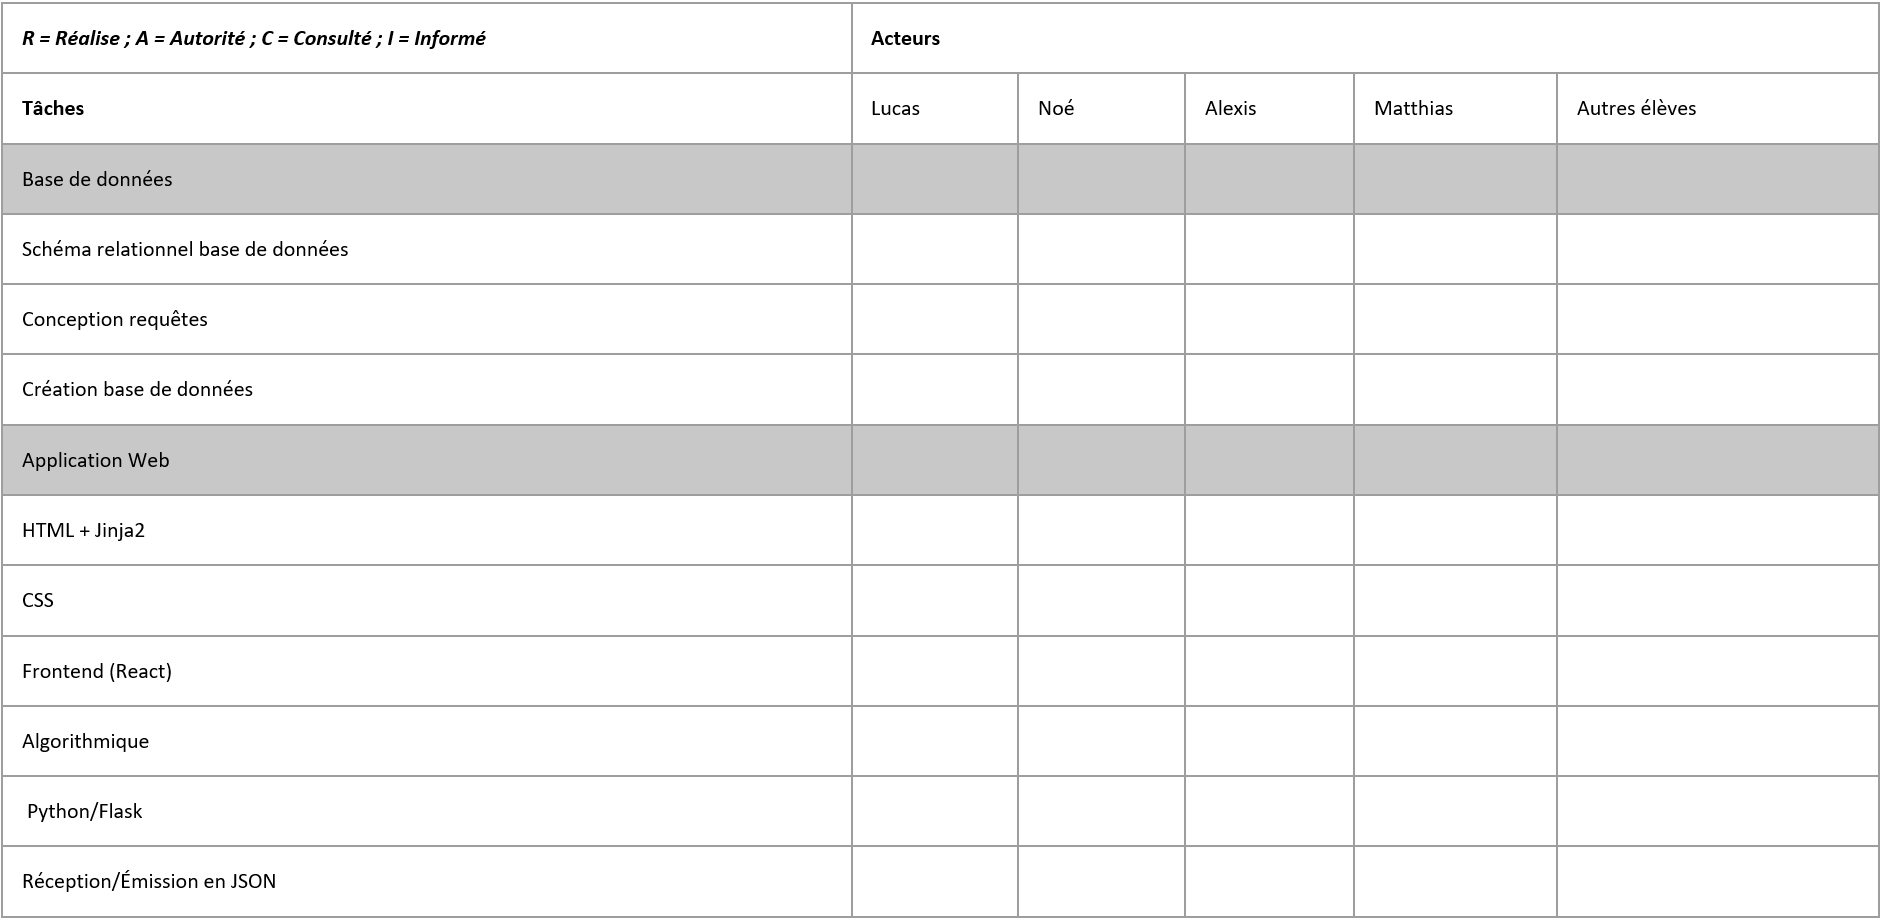
\includegraphics[width=0.75\textwidth]{img/RACI.png}
    \caption{Matrice RACI}
\end{figure} 

\newpage
\section{Application proposée}
\subsection{Définitions}
\textbf{Objectif général~: concevoir et d’implémenter une application innovante dédiées à l’optimisation des ressources dans les vergers et potagers du territoire.}

Notre application permet à un utilisateur de partager son jardin ou bien de rejoindre un jardin. Pour accéder aux fonctionnalités de l'application, l'utilisateur doit préalablement créer un compte.
Pour rejoindre un jardin, l'utilisateur a accès à une carte sur laquelle est affichée les jardins alentour.

Pour créer un jardin, l'utilisateur doit renseigner le nom et l'adresse du jardin. Il pourra ensuite rajouter diverses informations telles qu'une description et une photo par exemple. Un jardin a deux états possibles : public ou privé. Un jardin public apparait sur la carte et une demande pour rejoindre le jardin peut être faite par n'importe qui. A l'inverse un jardin privé peut seulement être rejoint via un lien d'invitation envoyé par le créateur.

Sur la page d'accueil, l'utilisateur a accès à tous ses jardins et peut accéder à la gestion de chacun d'entre eux. La gestion d'un jardin se fait principalement autour de la création d'une modélisation du plan réel du jardin par l'utilisateur. Sur cette modélisation, le créateur du jardin peut le séparer en plusieurs parties. Chaque partie est accompagnée d'un état, par exemple~: à semer, à labourer... Une partie est également accompagnée d'une liste des tâches à réaliser établis préalablement par les membres du jardin. Chaque tâche peut être validé par n'importe qui dans le jardin. De plus, on peut retrouver l'historique des tâches réalisées et par qui elles ont été réalisées.

Ces fonctionnalités permettent à un groupe de plusieurs personnes de s'organiser de manière dynamique et efficace.

\subsection{Fonctionnalités de l'application}
\begin{itemize}
    \item Compte~:
          \begin{itemize}
              \item Pour accéder aux fonctionnalités de l’application, une inscription sera nécessaire
          \end{itemize}
    \item Interactions d’un utilisateur avec les autres~:
          \begin{itemize}
              \item créer un jardin~:
                    \begin{itemize}
                        \item nom + adresse du jardin au minimum
                        \item deux états~:
                              \begin{itemize}
                                  \item public~: tout le monde peut voir le jardin sur la carte globale
                                  \item privé~: seul les membres du jardin peuvent le voir sur la carte globale
                              \end{itemize}
                    \end{itemize}
              \item rejoindre un jardin~:
                    \begin{itemize}
                        \item public~: tout le monde peut directement faire une demande qui sera accepter ou non par le créateur du jardin
                        \item privé~: un lien d’invitation envoyé par le créateur est nécessaire
                    \end{itemize}

          \end{itemize}
    \item fonctionnalités dans un jardin~:
          \begin{itemize}
              \item création d’une modélisation du plan réel du jardin~: création d’un jardin visuel suivant la forme du jardin réel
              \item  possibilité de diviser le jardin en plusieurs sous parties
              \item chaque partie du jardin a~:
                    \begin{itemize}
                        \item état (labouré, semé~: tomate, jachère…)
                        \item un liste des tâches à faire
                              \begin{itemize}
                                  \item intitulé de la tâche
                                  \item date limite de la tâche (optionnel)
                                  \item chaque tâche peuvent entre valider une fois faite
                              \end{itemize}
                        \item une historique des tâches qui ont été faite et par qui
                        \item possibilité de changer un état
                        \item possibilité d’ajouter,valider,supprimer des choses à faire
                    \end{itemize}
              \item vue global graphique des différents parties et états de chaque parties du jardin
          \end{itemize}
\end{itemize}
La création de la modélisation d’un jardin et de ses parties se fera de manière dynamique avec bloc graphique.

De même pour gérer l’état d’une partie, l’utilisateur pourra choisir le bloc qui correspond à son état et le glisser sur la partie du jardin correspondante.

\section{Conclusion}

\end{document}